\documentclass{article}
\usepackage[utf8]{inputenc}
\usepackage{amsmath}
\usepackage{amssymb}
\usepackage{amsthm}
\usepackage{enumerate}
\usepackage{mathtools}
\usepackage{float} % For plassering av bilder
\usepackage{a4wide} % mer width
\usepackage{amsmath}
\usepackage{amssymb}
\usepackage{parskip}
\usepackage{xcolor} % Fargelegger matriseelement
\usepackage{verbatim}
\usepackage{makecell} % formatere celler i tabell

\usepackage[colorlinks=false,allcolors=blue]{hyperref}
%Fikser hyperref
\addto\extrasnorsk{%
\def\figureautorefname{Figure}%
\def\tableautorefname{Table}%
\def\sectionautorefname{section}%
\def\subsectionautorefname{subsection}%
}
% Vi endrer fonten som brukes for URLer til den vanlige tekstfonten.
\urlstyle{same}


% FRA IC
\usepackage{natbib}
\usepackage{amsmath}
\usepackage{listings}
\usepackage{graphicx}

\usepackage[inline]{enumitem}
 \usepackage{booktabs}
\date{}
\newcommand*{\boxednumber}[1]{%
    \expandafter\readdigit\the\numexpr#1\relax\relax
}
\newcommand*{\readdigit}[1]{%
    \ifx\relax#1\else
        \boxeddigit{#1}%
        \expandafter\readdigit
    \fi
}
% Format macro used for every digit, adjust to your liking:
\newcommand*{\boxeddigit}[1]{\fbox{#1}\hspace{-\fboxrule}}

\usepackage[left=4cm,right=4cm,vmargin=1.5cm,footnotesep=0.5cm]{geometry}
\setlength\parindent{0pt}


\title{TDT4265 - Computer Vision and Deep Learning \\Assignment 3}
\author{Jakob Vahlin & Kristian Stensgård}
%\date{September 2020}

\begin{document}

\maketitle

\tableofcontents
\newpage

\section{Theory}

\subsection{Task 1a}

This subtask will discuss the spatial convolution of  an image, $\mathbf{P}$ with a kernel, $\mathbf{K}$ represented by the following $[3 \times5]$ and $[3\times3]$ matrices.

\begin{equation}
    \mathbf{P} = \begin{bmatrix}
        1 & 0& 2 & 3 & 1\\
          3 & 2& 0 & 7 & 0\\
         0 & 6& 1 & 1 & 4 \\
    \end{bmatrix}, \quad
    \mathbf{K} = \begin{bmatrix}
    -1 & 0 & 1 \\
    -2 &0& 2 \\
    -1 &0& 1 \\
    \end{bmatrix}
    \label{eq:image}
\end{equation}

It is desirable that the resulting convolved image, $\mathbf{C}$ has dimension $[3\times5]$. Using a stride length of 1, one \textit{layer} of zero padding must be added to the original image $\mathbf{P}$. The zero padded image, $\mathbf{P_z}$ will be represented by the following $[7\times5]$ matrix.  

\begin{equation}\def\r{\color{red}}\def\b{\color{blue}}
    \mathbf{P_z} = \begin{bmatrix}
    \r0 &\r0&\r0&\r0&\r0&\r0&\r0 \\
     \r 0&  1 & 0& 2 & 3 & 1&\r0\\
     \r 0&    3 & 2& 0 & 7 & 0&\r0\\
      \r0&   0 & 6& 1 & 1 & 4&\r0 \\
      \r0&\r0&\r0&\r0&\r0&\r0&\r0\\
    \end{bmatrix}
\end{equation}

Where the red zeros represent the zero padding. Thus the resulting operation will be to convolve the elements in $[3\times 3]$ ``sub matrcies'' of $\mathbf{P_z}$ with the kernel matrix, $\mathbf{K}$. To clarify what is meant by the term ``sub matrix'' equation \eqref{eq:demo} show the first and last sub matrices highlighted in blue. 

\begin{equation}\def\r{\color{red}}\def\b{\color{blue}}
    \mathbf{P_z} = \begin{bmatrix}
    \b0 &\b0&\b0&0&0&0&0 \\
     \b0&  \b1 & \b0& 2 & 3 & 1&0\\
      \b0&    \b3 & \b2& 0 & 7 & 0&0\\
      0&   0 & 6& 1 & 1 & 4&0 \\
      0&0&0&0&0&0&0\\
    \end{bmatrix}, \quad
    \mathbf{P_z} = \begin{bmatrix}
    0 &0&0&0&0&0&0 \\
     0&  1 & 0& 2 & 3 & 1&0\\
      0&    3 & 2& 0 &\b7 & \b0&\b0\\
      0&   0 & 6& 1 & \b1 & \b4&\b0 \\
      0&0&0&0&\b0&\b0&\b0\\
    \end{bmatrix}
    \label{eq:demo}
\end{equation}

With a stride length of 1, this blue square is shifted one step to the left (and one row down when the rightmost column has been reached) for each convolution with the kernel. The $j,k$th element in the convoled matrix $\mathbf{C}$, $c_{j,k}$ is given by

\begin{equation}
    c_{jk} = \sum_{l=0}^{3} \sum_{m=0}^{3} k_{l, m} a_{j+l, k+m} 
    \label{eq:conv}
\end{equation}
where $k_{l,m}$ represent the $l,m$th element in the Kernel matrix, $\mathbf{K}$ and $a_{x,y}$ represent the $x,y$th element in the zero padded input image, $\mathbf{P_z}$.


Thus from \eqref{eq:conv}, the element $c_{11}$ in the $\mathbf{C}$ matrix becomes

\begin{equation}
    c_{11} = 0(-1) + 0(0) + 0(1) + 0(-2) + 1(0) + 0(2) + 0(-1) + 3(0) + 2(1) = 2 
\end{equation}

Computing the rest of the elements in the following way finally gives the resulting covoluted image

\begin{equation}
    \mathbf{C} = \begin{bmatrix}
    2 &-1 & 11 &-2 &-13 \\
    10&-4 & 8 &2 &-18\\
    14 &-1 &-5 &6 &-9 \\
    \end{bmatrix}
\end{equation}


\begin{comment}
RIP THE PYTHON SCRIPT DREAM 
\begin{align}
    \begin{split}
      c_{11} (0)(-1) + (0)(-2) + (0)(-1) + (0)(0) + (1)(0) + (3)(0) + (0)(1) + (0)(2) + (2)(1) = 2\\
(0)(-1) + (1)(-2) + (3)(-1) + (0)(0) + (0)(0) + (2)(0) + (0)(1) + (2)(2) + (0)(1) = \\
(0)(-1) + (0)(-2) + (2)(-1) + (0)(0) + (2)(0) + (0)(0) + (0)(1) + (3)(2) + (7)(1) = \\
(0)(-1) + (2)(-2) + (0)(-1) + (0)(0) + (3)(0) + (7)(0) + (0)(1) + (1)(2) + (0)(1) = \\
(0)(-1) + (3)(-2) + (7)(-1) + (0)(0) + (1)(0) + (0)(0) + (0)(1) + (0)(2) + (0)(1) = \\
(0)(-1) + (0)(-2) + (0)(-1) + (1)(0) + (3)(0) + (0)(0) + (0)(1) + (2)(2) + (6)(1) = \\
(1)(-1) + (3)(-2) + (0)(-1) + (0)(0) + (2)(0) + (6)(0) + (2)(1) + (0)(2) + (1)(1) = \\
(0)(-1) + (2)(-2) + (6)(-1) + (2)(0) + (0)(0) + (1)(0) + (3)(1) + (7)(2) + (1)(1) = \\
(2)(-1) + (0)(-2) + (1)(-1) + (3)(0) + (7)(0) + (1)(0) + (1)(1) + (0)(2) + (4)(1) = \\
(3)(-1) + (7)(-2) + (1)(-1) + (1)(0) + (0)(0) + (4)(0) + (0)(1) + (0)(2) + (0)(1) = \\
(0)(-1) + (0)(-2) + (0)(-1) + (3)(0) + (0)(0) + (0)(0) + (2)(1) + (6)(2) + (0)(1) = \\
(3)(-1) + (0)(-2) + (0)(-1) + (2)(0) + (6)(0) + (0)(0) + (0)(1) + (1)(2) + (0)(1) = \\
(2)(-1) + (6)(-2) + (0)(-1) + (0)(0) + (1)(0) + (0)(0) + (7)(1) + (1)(2) + (0)(1) = \\
(0)(-1) + (1)(-2) + (0)(-1) + (7)(0) + (1)(0) + (0)(0) + (0)(1) + (4)(2) + (0)(1) = \\
(7)(-1) + (1)(-2) + (0)(-1) + (0)(0) + (4)(0) + (0)(0) + (0)(1) + (0)(2) + (0)(1) = \\
    \end{split}
\end{align}
\end{comment}
\subsection{Task 1b}

It is the convolution layer that gives a Convolutional Neural Network its translational invariance. This is a result of the fact that each convolutional layer uses the same \textit{kernel} (weights and biases). This means that all neurons in the convolutional layer detect the same \textit{feature} of the image that is fed into the network. Thus, if an image of i.e a cat were to be shifted some pixels to the left, the network would still be able to handle this, since the \textit{features} of the cat remains intact, and it is these features that will cause the activation of the neurons in a convolutional layer. What would happen is that the features describing the cat would be ``discovered'' a couple of pixels to the left. 


\subsection{Task 1c}

Given an image with height $H_1$ and width $W_1$, that is fed into a Convolutional Neural Network (CNN) with a stride of S, kernel size of $[F_H\times F_W]$, then height and with of the first convolutional layer is given by

\begin{align}
    H_2 &= \frac{H_1 - F_H + 2P_H}{S} + 1 \label{eq:h}\\ 
    W_2 &= \frac{W_1 - F_W + 2P_W}{S} + 1 \label{eq:w}
\end{align}
where $P_W$ and $P_H$ are the amount of zero-padding of the original image in the vertical and horizontal directions respectively.  

To determine what amount of zero-padding needed for the output shape of the convolutional layer to be equal to the input image for a CNN with stride, $S=1$, Kernel size of $[F_H = 5 \times F_W = 5]$, consider equations \eqref{eq:h} and \eqref{eq:w} with the values inserted.

\begin{align}
    H_2 &= H_2 - 5 + 2P_H + 1 \label{eq:ht}\\ 
    W_2 &= W_2 - 5 + 2P_W + 1 \label{eq:wt}
\end{align}
Note that $H_2 = H_1$ and $W_2 = W_1$, since the aim of the task is to achieve the same dimensions. Solving equations \eqref{eq:ht} and \eqref{eq:wt} w.r.t $P_H$ and $P_W$ respectively yields

\begin{align}
    \begin{split}
        2P_H &= H_2 - H_2 +5 -1 \\
        &= 5-1 \\ 
        &= 4 \\
        \implies P_H &=2
    \end{split}
    \begin{split}
        2P_W &= W_2 - W_2 +5 -1 \\
        &= 5-1 \\ &= 4 \\
        \implies P_W &=2
    \end{split}
\end{align}
Thus, \textbf{two} layers of zero padding, both in the width direction and height direction, is needed to achieve equal input and output dimensions. Thus, a $[m\times n]$ input matrix will be expanded to the dimensions $[m +4 \times n + 4]$, illustrated by the originally $[3\times 3]$, zero padded matrix shown in \eqref{eq:illu}
\begin{equation}\def\r{\color{red}}\def\b{\color{blue}}
    \mathbf{X_I} = \begin{bmatrix}
    \r0&\r0 &\r0&\r0&\r0&\r0&   \r0 \\
        \r0&\r0 &\r0&\r0&\r0&\r0    &\r0 \\
         \r0&\r 0&   a & b & c&\r0    &\r0\\
         \r0&\r 0&     d & e & f&\r0&    \r0 \\
          \r0&\r0&     g& h & i&\r0    &\r0 \\
          \r0&\r0&\r0&\r0&\r0&\r0    &\r0\\
                    \r0&\r0&\r0&\r0&\r0&\r0   & \r0\\
    \end{bmatrix}
    \label{eq:illu}
\end{equation}
where red zeros indicate the zero-padding.

\subsection{Task 1d} \label{sec:t1d}
For this task, formula describing the dimensions of the layers in the network in equations \eqref{eq:h} and \eqref{eq:w} can again be used. For a network whose inputs are RGB colored images with dimensions $[H_1 = 514 \times W_1 = 514]$ without zero padding, and the feature maps in the first hidden convoluted layer are of dimensions $[H_2 = 504 \times W_2 = 504]$ with stride, $S=1$, equations \eqref{eq:h} and \eqref{eq:w} becomes 

\begin{align}
    504 &= 512 - F_H + 0 + 1 \\
    504 &= 512 - F_W + 0 + 1
\end{align}
Solving for $F_H$ and $F_W$ yields

\begin{align}
    \begin{split}
        504 &= 512 - F_H + 0 + 1 \\
        \implies F_H &= 9
    \end{split}
    \begin{split}
        504 &= 512 - F_W + 0 + 1 \\
        \implies F_W &= 9
    \end{split}
\end{align}

Thus the Kernels are of dimensions $[9\times 9]$.

\subsection{Task 1e}
Subsampling and pooling will produce feature maps of size $H \times W$ given by the same formulas for convolution, i.e \autoref{eq:h} and \autoref{eq:w}. From  task 1d the output of the first convolutional layer has dimensions $504 \times 504$. This is the input to the subsampling, and with a stride $S=2$ with a neighbourhood(kernel?)  $F = 2 \times 2$. The padding $P$ is zero. Since the kernel is square and the input is square, the resulting feature map will also be square. Solving \autoref{eq:h} for the subsampling gives:


\begin{align}
\begin{split}
    H_2 &= \frac{504 -2 + (2\cdot 0)}{2}  +1 \\
    H_2 &= 252
    \implies W_2 = 252
\end{split}
\end{align}

The spatial dimensions after the pooling is $ 252 \times 252$ 

\subsection{Task 1f}
For this task the same equations used in the three previous tasks will be used, namely \autoref{eq:h} and \autoref{eq:w}. With subsampling between the two convolutional layers the input to the second convolutional layer has spatial dimensions $252 \times 252$. Using the same equations as previously, the output dimensions are:

\begin{align}
\begin{split}
    H_2 = \frac{252 -3 + (2\cdot0)}{1}  +1 \\
    H_2 = 250
    \implies W_2 = 250
\end{split}
\end{align}

The spatial dimensions after the second convolution are $250 \times 250$

\subsection{Task 1g}
The network specified in the assignment consists of 3 convolutional layers with a kernel with dimensions $ 5\times 5$ and 32, 64 and 128 filters respectively. Lastly there is two fully connected layers with $64$ and $10$ hidden units.

The number of parameters in a convolutional layer is the total number of filters, times the number of parameters for each kernel associated with the filter. The number of parameters for a kernel is the kernel size plus a bias. 

For the first layer in the network, there is a total of 32 filters. This means that there are 32 sets of unique weights and biases. Since the input image have 3 colour channels (RGB) and we have a square kernel of $5 \times 5$, the weights have $(5 \cdot 5 \cdot 3) +1 = 76$ parameters, the $ +1$ is the bias. This results in $76 \cdot 32 = 2432$ parameters for the first layer. 
Doing this for the rest of the network we get:

\begin{align}
    \begin{split}
    (5 \cdot 5 \cdot 32) +1) \cdot 64 = 51,264 \\ % layer 2
    (5 \cdot 5 \cdot 64) +1) \cdot 128 = 204,928 % layer 3
    \end{split}
\end{align}



For the fully connected layers we have one weight matrix per layer with dimensions defined by the input layer and the number of hidden units in the layer. The spatial dimensions in each feature map after the last convolutional layer is $4 \times 4$ this follows from calculations using the same approach as in the previous tasks. Additionally, there are biases in the input and hidden layer of the fully connected network. Thus the input dimension is increased by one. This gives


\begin{align}
\begin{split}
    ((128 \cdot 4 \cdot 4) +1) \cdot 64 = 131,136 \\
    (64+1) \cdot 10 = 650
\end{split}
\end{align}


Thus the total number of parameters in the network is:

\begin{equation}
    2432 + 51,264 + 204,928 + 131,136 + 650 = 390,410
\end{equation}


\section{Task 2}
In this task a Convolutional Neural Network has been implemented and trained on the CIFAR-10 dataset, with 50,000 training images and 10,000 test images. $10\%$ of the training images has been used as a validation set and was not used for the training. The network is described in \autoref{tab:networktask2}.

\subsection{Task 2a \& 2b: Training and validation loss and accuracy.}

The network was trained on the CIFAR-10 dataset. A plot of the resulting training and validation loss as well as the validation accuracy is shown in \autoref{fig:task2_loss} and \autoref{fig:task2_acc}.

The network had a minimum validation loss of $0.85$ and a peak validation accuracy of $74.6\%$. After training the model a average loss of $0.798$ and average accuracy of $73.8\%$ was acheived on the test set using the same version of the network that got the best performance on the validation set. For the training set the average loss was $0.369$ and the average accuracy was $87.7\%$ when the trained network was used. 

\begin{table}[H]
\centering
\caption{Description of the CNN in task 2.}
\label{tab:networktask2}
\begin{tabular}{c|c|c|c}
\textbf{Layer} & \textbf{Layer Type} & \textbf{Number of Hidden Units} & \textbf{Activation Function} \\ \hline
1 & Conv2D & 32 & ReLU \\
1 & MaxPool2D & - & - \\
2 & Conv2D & 64 & ReLU \\
2 & MaxPool2D & - & - \\
3 & Conv2D & 128 & ReLU \\
3 & MaxPool2d & - & - \\ \hline
 & Flatten & - & - \\
4 & Fully-Connected & 64 & ReLU \\
5 & Fully-Connected & 10 & Softmax
\end{tabular}
\end{table}


\begin{figure}[H]
    \centering
    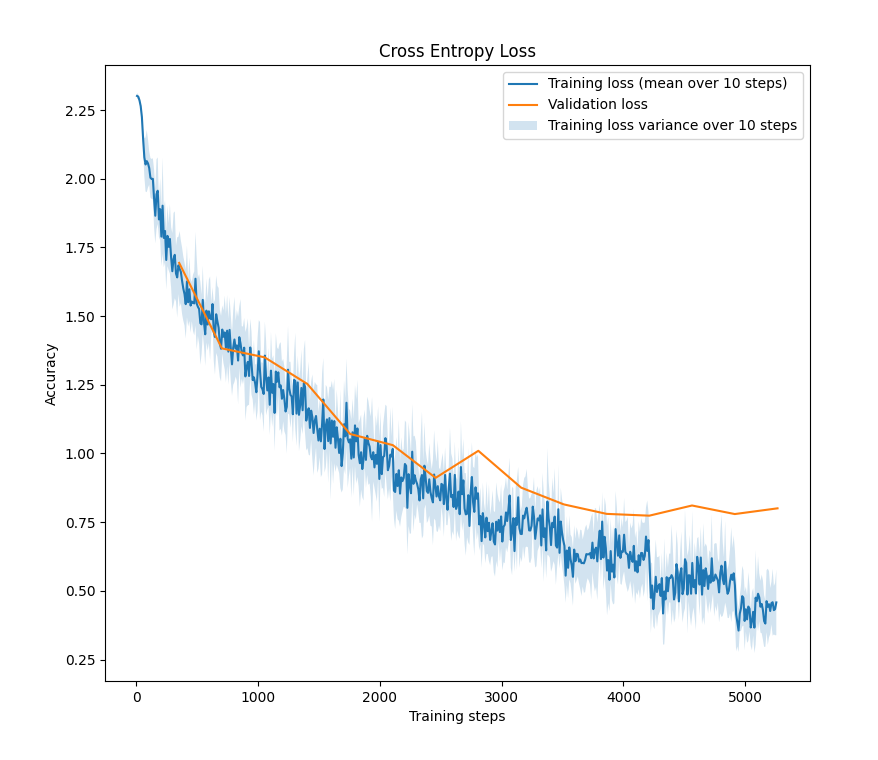
\includegraphics[width = \textwidth]{Assignments/Assignment_3/plots/ass_3_task2_loss.png}
    \caption{Training and validation loss for the network during training.}
    \label{fig:task2_loss}
\end{figure}

\begin{figure}[H]
    \centering
    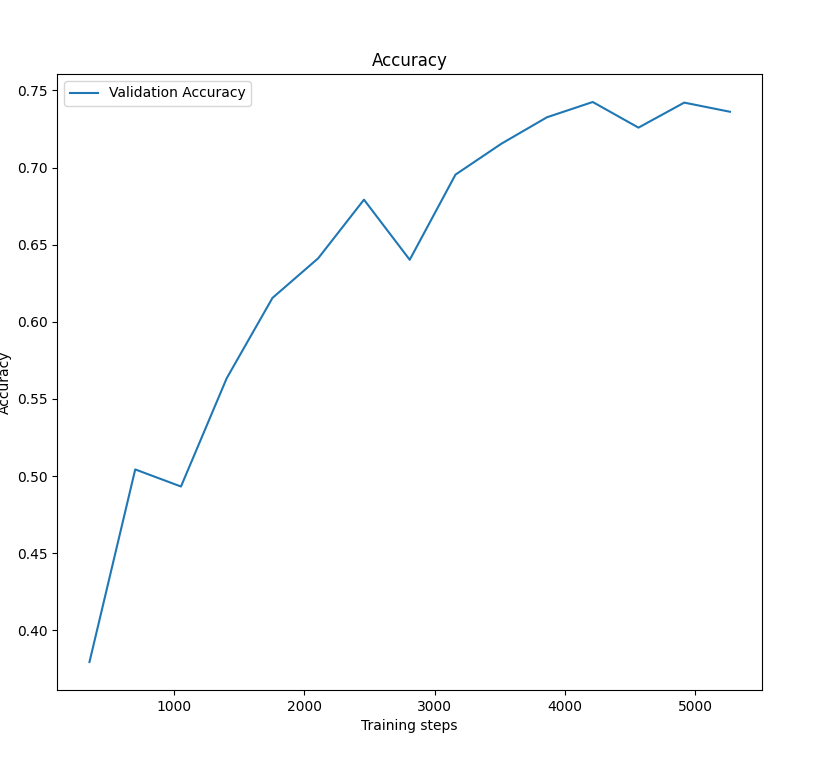
\includegraphics[width = \textwidth]{Assignments/Assignment_3/plots/ass_3task_2_acc.png}
    \caption{Validation accuracy for the network during training.}
    \label{fig:task2_acc}
\end{figure}

From the plot of the resulting cross entropy loss shown in \autoref{fig:task2_loss} one can observe that the validation loss seems to be on an upward trend as the training stops. This upward trend could be a sign of the model starting to overfit. Additionally the training loss tends towards zero, creating a ``gap'' between the validation and training loss, which supports the claim of overfitting.

\section{Task 3}

This task adresses the design of two different Convulotional Neural Networks using different architectures, hyperparameters, loss functions, and optimizers. 

\subsection{Task 3a: Description of the networks}

A description of Network 1 is given in \autoref{tab:network1}. Each convolutional layer has filter size of $[5\times 5]$, with a padding of 2 and a stride of 1. The flatten layer takes an image with shape (Height) $\times$ (Width) $\times$ (Number of Feature Maps), and flattens
it to a single vector with size (Height) $\cdot$ (Width) $\cdot$ (Number of Feature Maps).  The MaxPool layers have filters with size $[2\times2]$, stride of 2 and no zero-padding.

The training details of Network 1 are outlined in \autoref{tab:net1trainparam}. In addition to the details outline in \autoref{tab:net1trainparam}, data augmentation on the input data was used. The input images were cropped randomly, meaning that a random selection of the image was chosen and padding added to keep the dimensions intact. ``Random horizontal flip'' was also added, meaning that there was a 50\% chance of the image being mirrored.   

\begin{table}[H]
\centering
\caption{The network architecture of Network 1. (task3_network1.py)}
\label{tab:network1}
\begin{tabular}{c|c|c|c}
\textbf{Layer} & \textbf{Layer Type} & \textbf{Number of Hidden Units} & \textbf{Activation Function} \\ \hline
1 & Conv2D & 32 & ReLU \\
1 & BatchNorm2D & - & - \\
2 & Conv2D & 64 & ReLU \\
2 & MaxPool2D & - & - \\
3 & Conv2D & 128 & ReLU \\
3 & BatchNorm2D & - & - \\
4 & Conv2D & 128 & ReLU \\
4 & Maxpool2D & - & - \\
4 & Dropout2D & - & - \\\hline

 & Flatten & - & - \\
5 & Fully-Connected & 64 & ReLU \\
5 & BatchNorm1D & - & - \\
5 & Dropout & - & - \\
6 & Fully-Connected & 64 & ReLU \\
6 & BatchNorm1D & - & - \\
6 & Dropout & - & - \\
7 & Fully-Connected & 64 & ReLU \\
7 & BatchNorm1D & - & - \\
7 & Dropout & - & - \\
8 & Fully-Connected & 64 & ReLU \\
8 & BatchNorm1D & - & - \\
8 & Dropout & - & - \\
8 & Fully-Connected & 10 & SoftMax \\
\end{tabular}
\end{table}

% Please add the following required packages to your document preamble:
% \usepackage{graphicx}
\begin{table}[H]
\centering
\caption{Training parameters used when training Network 1.}
\label{tab:net1trainparam}
\resizebox{\textwidth}{!}{%
\begin{tabular}{|l|l|l|l|l|l|l|}
\hline
\textbf{Optimizer} & \textbf{Regularization} & \textbf{Batch size} & \textbf{Learning rate} & \textbf{Weight Init} & \textbf{Epochs} & \textbf{Early stop count} \\ \hline
SGD               & Dropout, rate = 0.05    & 64                  & 0.04                   & Uniform              & 10              & 4                         \\ \hline
\end{tabular}%
}
\end{table}

A description of Network 2 is given in \autoref{tab:network2}. Each convolutional layer has filter size of $[3\times 3]$, with a padding of 2 and a stride of 1. The flatten layer takes an image with shape (Height) $\times$ (Width) $\times$ (Number of Feature Maps), and flattens
it to a single vector with size (Height) $\cdot$ (Width) $\cdot$ (Number of Feature Maps). The MaxPool layers have filters with size $[2\times2]$, stride of 2 and no zero-padding.

The training details of Network 2 are outlined in \autoref{tab:net2trainparam}. In addition to the details outline in \autoref{tab:net2trainparam}, data augmentation on the input data was used. The input images were cropped randomly, meaning that a random selection of the image was chosen and padding added to keep the dimensions intact. ``Random horizontal flip'' was also added, meaning that there was a 50\% chance of the image being mirrored.   

\begin{table}[H]
\centering
\caption{The network architecture of Network 2. (task3\_3.py)}
\label{tab:network2}
\begin{tabular}{c|c|c|c}
\textbf{Layer} & \textbf{Layer Type} & \textbf{Number of Hidden Units} & \textbf{Activation Function} \\ \hline
1 & Conv2D & 32 & ReLU \\
2 & Conv2D & 64 & ReLU \\
2 & BatchNorm2D & - & - \\
2 & MaxPool2D & - & - \\
3 & Conv2D & 128 & ReLU \\
3 & BatchNorm2D & - & - \\
3 & MaxPool2D & - & - \\
3 & Dropout & - & - \\\hline
 & Flatten & - & - \\
5 & Fully-Connected & 64 & ReLU \\
5 & BatchNorm1D & - & - \\
8 & Fully-Connected & 10 & SoftMax \\
\end{tabular}
\end{table}

% Please add the following required packages to your document preamble:
% \usepackage{graphicx}
\begin{table}[]
\centering
\caption{Training parameters used when training Network 2.}
\label{tab:net2trainparam}
\resizebox{\textwidth}{!}{%
\begin{tabular}{|l|l|l|l|l|l|l|}
\hline
\textbf{Optimizer} & \textbf{Regularization} & \textbf{Batch size} & \textbf{Learning rate} & \textbf{Weight Init} & \textbf{Epochs} & \textbf{Early stop count} \\ \hline
SGD               & Dropout, rate = 0.1     & 64                  & 0.05                   & Uniform              & 10              & 4                         \\ \hline
\end{tabular}%
}
\end{table}




\subsection{Task 3b: Loss and accuracy results}

The resulting final train loss, final train accuracy, final validation accuracy and average test accuracy for the two networks are outlined in \autoref{tab:3b_results}

\begin{table}[H]
\centering
\caption{Final train loss, final train accuracy, final validation accuracy and average test accuracy for the two networks.}
\label{tab:3b_results}
\resizebox{\textwidth}{!}{%
\begin{tabular}{|l|l|l|l|l|}
\hline
\textbf{Model} & \textbf{Train loss} & \textbf{Train accuracy} & \textbf{Validation accuracy} & \textbf{Test accuracy} \\ \hline
Network 1      & 0.605                     & 79.5 \%                       & 79.1 \%                            & 78.6 \%                        \\ \hline
Network 2      & 0.546                     & 80.1 \%                       & 78.4 \%                            & 77.5 \%                        \\ \hline
\end{tabular}%
}
\end{table}

The validation accuracy and training and validation loss from the best model, Network 1, are shown in \autoref{fig:task3bbest_acc} and \autoref{fig:task3bbest_loss} respectively.  

\begin{figure}[H]
    \centering
    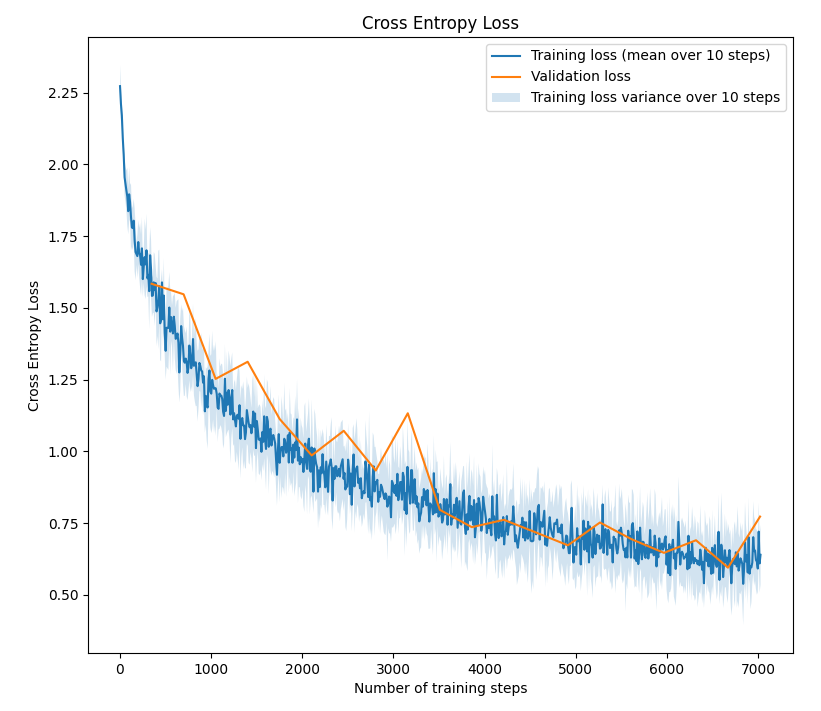
\includegraphics[width = \textwidth]{Assignments/Assignment_3/plots/task3best_plot_loss.png}
    \caption{Training and validation loss for Network 1.}
    \label{fig:task3bbest_loss}
\end{figure}



\begin{figure}[H]
    \centering
    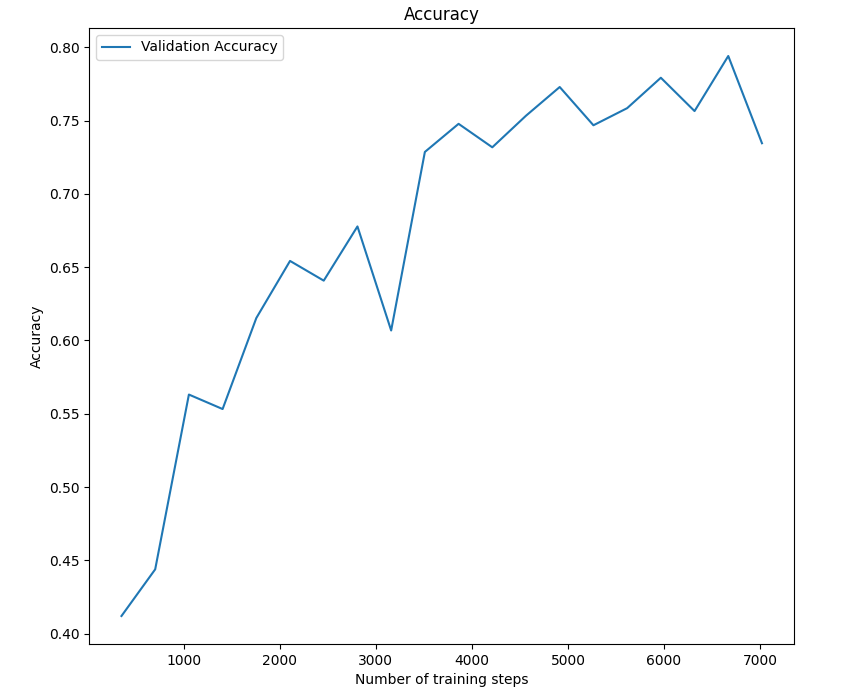
\includegraphics[width =\textwidth]{Assignments/Assignment_3/plots/task3best_plot_accuracy.png}
    \caption{Validation accuracy for Network 1.}
    \label{fig:task3bbest_acc}
\end{figure}

\subsection{Task 3c: Useful methods}

In an attempt to improve the networks performance, several different additions and alterations was done:

A lot of time was spent testing different network architectures. Both different number of filters, hidden units, and number of layers. After data augmentation, the network architecture was the most impactful. Overall, deeper networks, with more filters and more convolutional layers gave more successful results. However, if the networks became too deep, the results became worse. This is to be expected, as deeper netwtorks initially gives the model a better chance of improving on classifying the details, but if the network becomes too deep, the gradients will ``vanish'', and the model grows way too large for it to be possible to perform valuable training.  


The most impactful increase in performance came after adding data augmentation. The performance increase can probably be explained by the fact that data augmentation slightly changes the input images. This creates a more diverse training set, resulting in a more robust model. However, augmenting the data too much gave worse results, probably due to the fact that changing the input \textit{too} much creates a training set that is \textit{too} diverse, and thus the model is unable to recognize patterns and draw worthy conclusions. 

Different activation functions was tested including, tanh, sigmoid and leaky ReLU. However they did not improve the performance of the network. When testing these activation functions, different weight initializations was also tested to match the activation functions. The lack of success from the tanh and sigmoid activation functions could be a explained by their known issues with vanishing gradients.

Batch normalization seemed to have little to no effect on the performance of the network, altough the technique was not tested extensively. This might be a consequence of the ``heavy'' data augmentation used on the input data, meaning that batch normalizing will have little effect on the training of the network.  

The Adam optimizer was tested in favour of SGD, but it didn't improve the performance of the network at the end of training, but it converged at approximately the same rate as SGD in the beginning. This is a well known fact for the Adam optimizer. In hindsight a weight decay could be added to the Adam optimizer and maybe improve the performance. 
% WÅNK setning

Experiments with dropout showed that it helps to reduce overfitting, but it should be used carefully as too much dropout resulted in very poor performance. This could be because if the model has a high drop out rate (meaning fewer connections between the layers, and fewer weights, resulting in a less comprehensive model), it missed out on some important characteristics that it might have learned about had it not had such a high drop out rate, leading to more generalization.

\subsection{Task 3d: Illustrating the impact of most useful addition}

The most impactful addition turned out to be the implementation of data augmentation. To illustrate the impact, the resulting train and validation loss before and after the implementation for Network 1, is shown in \autoref{fig:wwdataaug}

\begin{figure}[H]
    \centering
    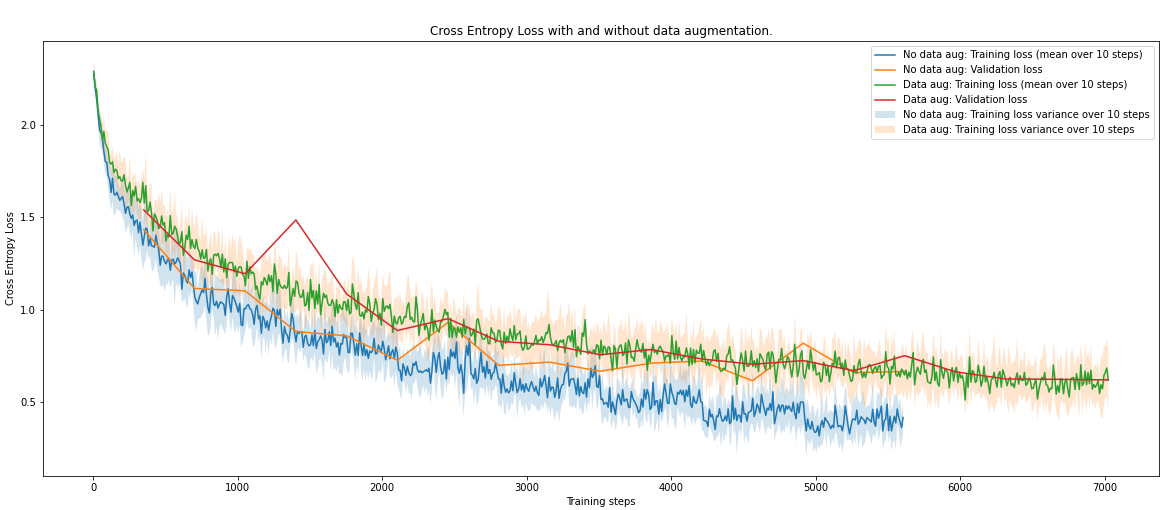
\includegraphics[width = \textwidth]{Assignments/Assignment_3/plots/task3d_plot.png}
    \caption{Training and validation loss with and without data augmentation.}
    \label{fig:wwdataaug}
\end{figure}



\subsection{Task 3e: Improving the best network}

The best model from task 3a, Network 1, was further developed with the aim of reaching a test accuracy of more than 80\%. In an effort to increase the test accuracy, the data augmentation was modified. The random cropping that was previously used, was removed and instead a random rotation of the image was introduced. Random rotation will rotate the image with a degree drawn uniformly from the range $[-10, 10]$.

In addition to the modified data augmentation, the learning rate was reduced from $4\cdot 10^{-2}$ to $3.5 \cdot 10^{-2}$.

The network architecture remained mostly unchanged. However, dropout was removed from the fully connected network when performing classification.

A description of the improved network is given in \autoref{tab:network_improved}. The modified training details are outlined in \author{tab:netimprovedtrainparam}.

With these changes implemented the network reached an average accuracy of$80.5\%$ on the test set. The performance metrics for the improved metrics are outlined in \autoref{tab:3e_results}.

\begin{table}[H]
\centering
\caption{The network architecture of the improved network. (task3.py)}
\label{tab:network_improved}
\begin{tabular}{c|c|c|c}
\textbf{Layer} & \textbf{Layer Type} & \textbf{Number of Hidden Units} & \textbf{Activation Function} \\ \hline
1 & Conv2D & 32 & ReLU \\
1 & BatchNorm2D & - & - \\
2 & Conv2D & 64 & ReLU \\
2 & MaxPool2D & - & - \\
3 & Conv2D & 128 & ReLU \\
3 & BatchNorm2D & - & - \\
4 & Conv2D & 128 & ReLU \\
4 & Maxpool2D & - & - \\
4 & Dropout2D & - & - \\\hline

 & Flatten & - & - \\
5 & Fully-Connected & 64 & ReLU \\
5 & BatchNorm1D & - & - \\
6 & Fully-Connected & 64 & ReLU \\
6 & BatchNorm1D & - & - \\
7 & Fully-Connected & 64 & ReLU \\
7 & BatchNorm1D & - & - \\
8 & Fully-Connected & 64 & ReLU \\
8 & BatchNorm1D & - & - \\
8 & Fully-Connected & 10 & SoftMax \\
\end{tabular}
\end{table}

% Please add the following required packages to your document preamble:
% \usepackage{graphicx}
\begin{table}[H]
\centering
\caption{Training parameters used when training the improved network.}
\label{tab:netimprovedtrainparam}
\resizebox{\textwidth}{!}{%
\begin{tabular}{|l|l|l|l|l|l|l|}
\hline
\textbf{Optimizer} & \textbf{Regularization} & \textbf{Batch size} & \textbf{Learning rate} & \textbf{Weight Init} & \textbf{Epochs} & \textbf{Early stop count} \\ \hline
SGD               & Dropout, rate = 0.05    & 64                  & 0.035                   & Uniform              & 10              & 4                         \\ \hline
\end{tabular}%
}
\end{table}

% Please add the following required packages to your document preamble:
% \usepackage{graphicx}
\begin{table}[H]
\centering
\caption{Final train loss, final train accuracy, final validation accuracy and average test accuracy for the improved network}
\label{tab:3e_results}
\resizebox{\textwidth}{!}{%
\begin{tabular}{|l|l|l|l|l|}
\hline
\textbf{Model} & \textbf{Train loss} & \textbf{Train accuracy} & \textbf{Validation accuracy} & \textbf{Test accuracy} \\ \hline
Improved       & 0.458                     & 84.2 \%                       & 79.5                               & 80.6 \%                        \\ \hline
\end{tabular}%
}
\end{table}

\begin{figure}[H]
    \centering
    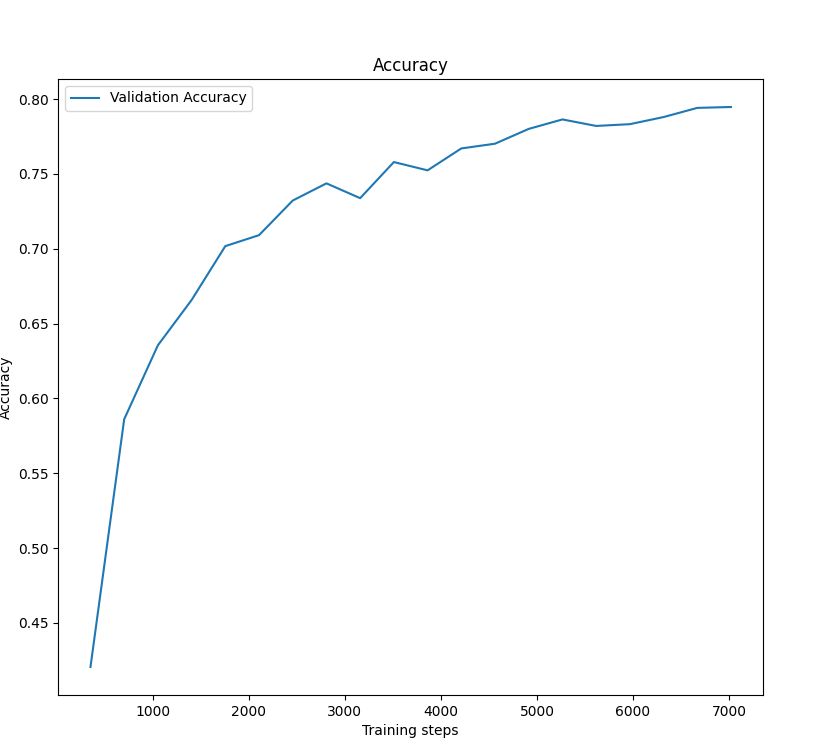
\includegraphics[width = \textwidth]{Assignments/Assignment_3/plots/task3e_plot.png}
    \caption{Validation accuracy for the improved model.}
    \label{fig:valaccimproved}
\end{figure}

\subsection{Task 3f: Signs of overfitting}

From the plot of the resulting cross entropy loss shown in \autoref{fig:improved_loss} one can observe that the validation loss follows the loss for the training set. The validation loss is flattening a bit more than the training set. This not a direct sign of overfitting yet, as the ``gap'' between the two loss lines is not very significant.  

\begin{figure}[H]
    \centering
    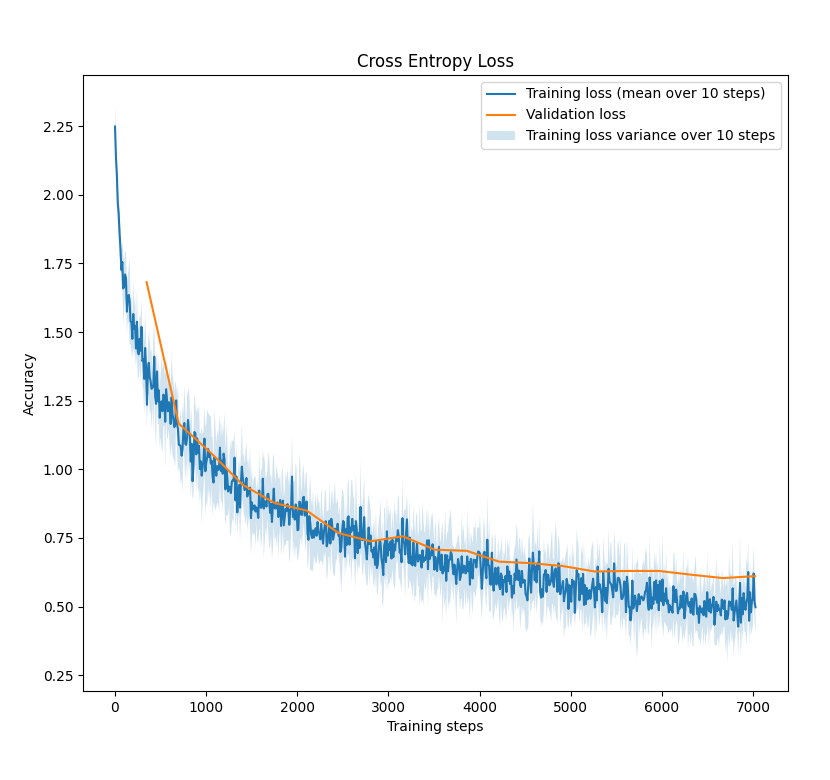
\includegraphics[width = \textwidth]{Assignments/Assignment_3/plots/painteroooo.png}
    \caption{The training and validation loss for the improved network.}
    \label{fig:improved_loss}
\end{figure}

\section{Task 4: : Transfer Learning with ResNet}

\subsection{Task 4a: Transfer learning with ResNet18}

In this task a pre-trained version of ResNet called ResNet18 is used with the same training, validation and test sets as used in task 2 and task 3. The network is trained with the Adam optimizer with a learning rate of $5 \cdot 10 ^{-4}$ and a batch size of 32. The only data augmentation that was used was resizing the images to be correct size for the network and normalising. The network is trained for $4$ epochs before early stopping kicks in. 

The performance metrics of the network are shown in \autoref{tab:pre-train}. \autoref{fig:4aloss} show plots of the Cross Entropy Loss for both validation and training sets. \autoref{fig:4aacc} show plot of the validation accuracy.

\begin{table}[H]
\centering
\caption{Loss and accuracy for the training, validation and testing sets}
\label{tab:pre-train}
\begin{tabular}{|l|l|l|}
\hline
\textbf{Dataset} & \textbf{Loss} & \textbf{Accuracy} \\ \hline
Training set     & 0.52          & 82.7 \%           \\ \hline
Validation set   & 0.48          & 84.3 \%           \\ \hline
Test set      & 0.55          & 82.0 \%           \\ \hline
\end{tabular}
\end{table}

\begin{figure}[H]
    \centering
    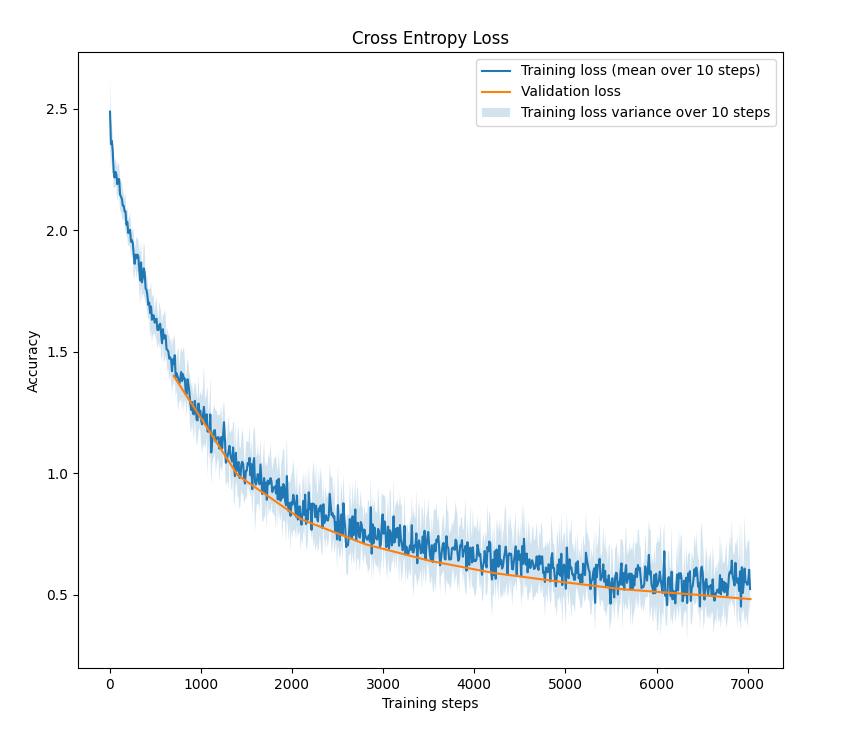
\includegraphics[width=\textwidth]{Assignments/Assignment_3/plots/task4a_plot_loss.png}
    \caption{Training and validation loss for ResNet18.}
    \label{fig:4aloss}
\end{figure}

\begin{figure}[H]
    \centering
    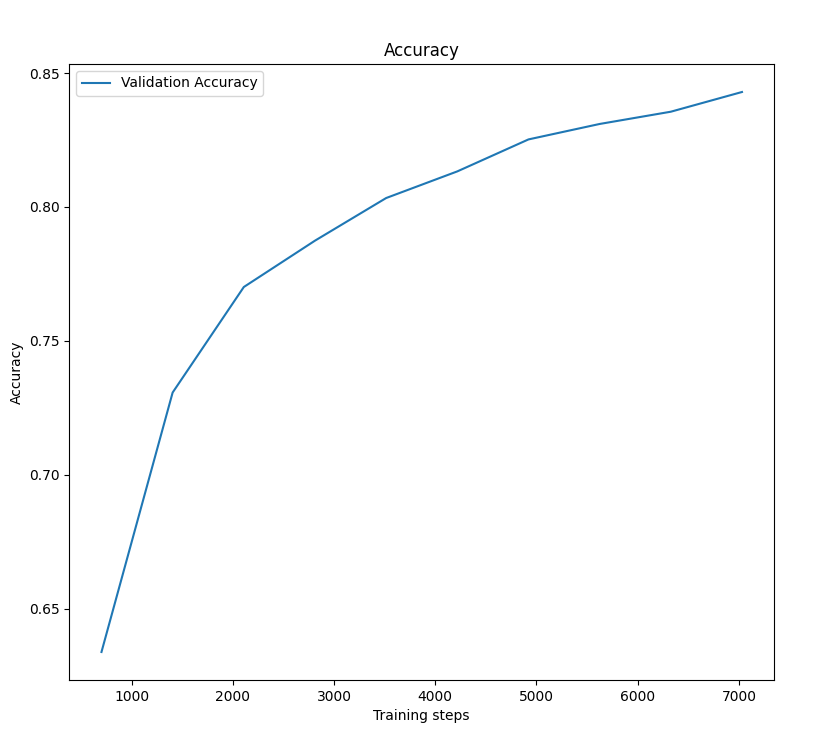
\includegraphics[width = \textwidth]{Assignments/Assignment_3/plots/task4a_plot_acc.png}
    \caption{Validation accuracy for ResNet18}
    \label{fig:4aacc}
\end{figure}




As we see from the results the pre-trained network performs way better than the networks in task 2 and task 3. Even with less training time on the CIFAR10 dataset.  







\subsection{Task 4b: Filter visualization}
To visualize the feature extraction done by the filters, the weights and activation of the filters in the first convolutional layer of the trained model have been investigated. The image used as an example is an image of a zebra, shown in \autoref{fig:zebra}. The feature extraction, beeing the weights and convolution outputs, from the filters in the first convolutional layer in the pretrained model is visualized in \ref{fig:zebra_feature}.

It is clear from \autoref{fig:zebra_feature} that the two first weights detect vertical and horizontal lines using weights that resembles the Sobel kernel. The fourth kernel appears to detect diagonal lines, while the third and fifth kernel appears to be bell shapes meant to detect a specific colour. 

\begin{figure}[H]
    \centering
    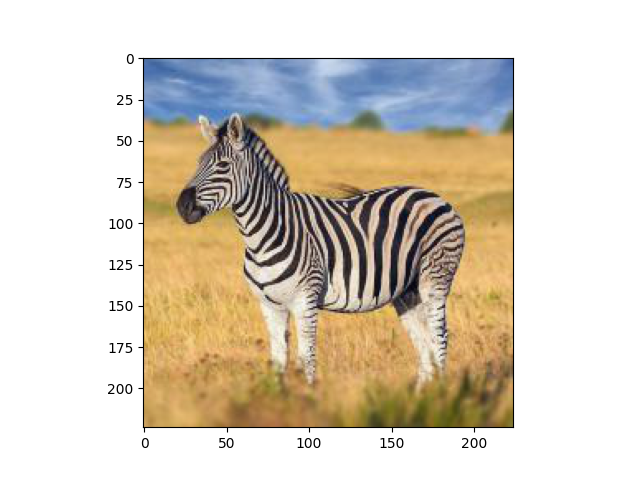
\includegraphics[width=\textwidth]{Assignments/Assignment_3/plots/zebra.png}
    \caption{An image of a Zebra used when visualizing the feature extraction of the filters in the first convolutional layer.}
    \label{fig:zebra}
\end{figure}

\begin{figure}[H]
    \centering
    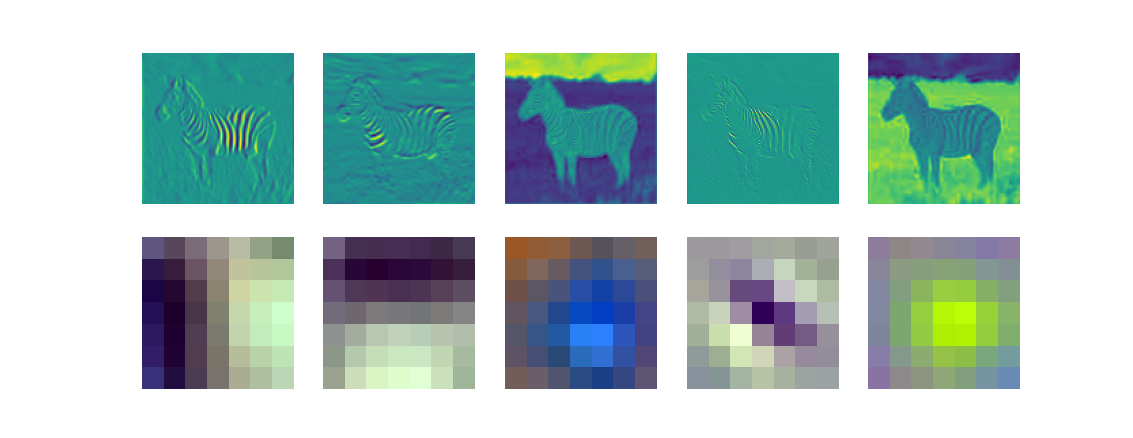
\includegraphics[width=\textwidth]{Assignments/Assignment_3/plots/zebra_all.png}
    \caption{Feature extraction of from filters in the first convolutional layer. Top row: The convolution outputs. Bottom row: The corresponding weights that produced the output.}
    \label{fig:zebra_feature}
\end{figure}




\subsection{Task 4c}
For this task the activations from the very last convolutional layer in ResNet18 is plotted in \autoref{fig:activations}. From looking at the activations themselves it is hard to find out what features the network has extracted. However by overlaying the input image as seen in \autoref{fig:activationszebra}, we see that the network puts emphasis on the legs and on the head of the zebra. 
\begin{figure}[H]
    \centering
    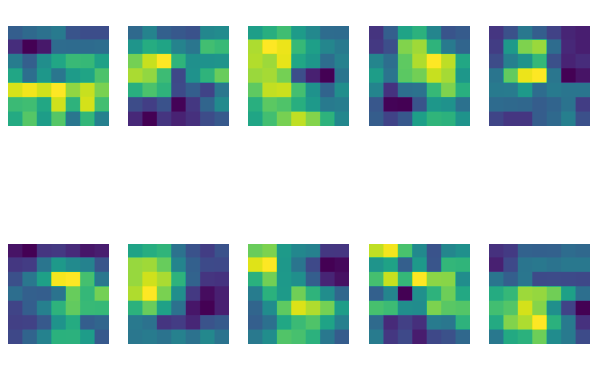
\includegraphics[width=\textwidth]{Assignments/Assignment_3/plots/activationsc4c.png}
    \caption{Activations from the last convolutional layer in ResNet18}
    \label{fig:activations}
\end{figure}


\begin{figure}[H]
    \centering
    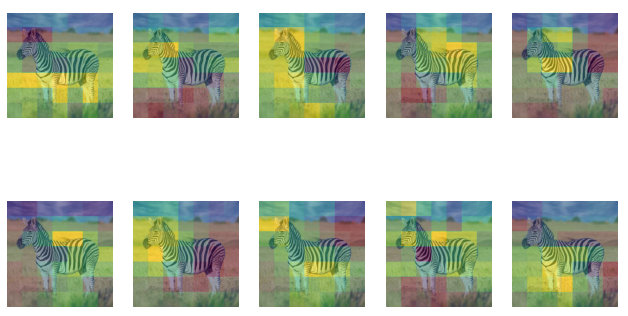
\includegraphics[width=\textwidth]{Assignments/Assignment_3/plots/activations4c_zebrac.png}
    \caption{Activations from the last convolutional layer in ResNet18 oberlayed on the input image}
    \label{fig:activationszebra}
\end{figure}



% Reffe stanford?
% \begin{thebibliography}{9}
% \bibitem{sauce}
% [LeCun et al., 2012] LeCun, Y. A., Bottou, L., Orr, G. B., and Müller, K.-R. (2012). Efficient backprop.
% \textit{In Neural networks: Tricks of the trade}, pages 9–48. Springer.
% \end{thebibliography}
\end{document}